\section{Introduzione}
    \subsection{Reti Di Calcolatori}
        Una \textit{rete di calcolatori} è una rete di nodi di elaborazione:
        \begin{itemize}
            \item Totalmente autonomi tra loro
            \item Connessi mediante un opportuno sistema di comunicazione
            \item In grado di interagire mediante scambio di messaggi
        \end{itemize}
    
    \subsection{Componenti della comunicazione}
        La comunicazione avviene attraverso canali individuati sulla rete da cinque componenti:
        \begin{enumerate}
            \item \textit{Mesaggio}: informazione da trasferire.
            \item \textit{Mittente}: dispositivo che spedisce il messaggio.
            \item \textit{Destinatario}: dispositivo che riceve il messaggio.
            \item \textit{Mezzo di trasmissione}: cammino fisico percorso dal messaggio.
            \item \textit{Protocollo}: insieme di regole che governano la comunicazione.
        \end{enumerate}
    
    \subsection{Valutazione del canale di comunicazione}
        Un canale di comunicazione viene valutato in base a:
        \begin{itemize}
            \item \textit{Ampiezza di banda}: capacità teorica del canale, espressa in bit/sec.
            \item \textit{Throughput}: capacità misurata del canale, espressa in bit/sec.
            \item \textit{Latenza}: tempo di trasferimento di un bit da un canale all'altro, espresso in sec.
            \item \textit{Jitter}: variazione della latenza.
            \item \textit{Affidabilità}: intolleranza agli errori di trasmissione, percentuale di bit persi.
            \item \textit{Sicurezza}: capacità di opporsi ad accesso non autorizzato, danno o violazioni della rete.
        \end{itemize}

        \begin{table}[ht]
            \centering
            \begin{tabular}{|c|c|c|c|c|}
                \hline
                Applicazione & Affidabilità & Latenza & Jitter & Banda \\
                \hline
                E-mail & Alta & Bassa & Basso & Bassa \\
                \hline
                Trasferimento file & Alta & Bassa & Basso & Media \\
                \hline
                Accesso web & Alta & Media & Basso & Media \\
                \hline
                Login remoto & Alta & Media & Medio & Bassa \\
                \hline
                Audio on-demand & Bassa & Bassa & Alto & Media \\
                \hline
                Video on-demand & Bassa & Bassa & Alto & Alta \\
                \hline
                Telefonia & Bassa & Alta & Alto & Bassa \\
                \hline
                Videoconferenza & Bassa & Alta & Alto & Alta \\
                \hline
            \end{tabular}
            \caption*{1.a: Tabella di valutazione applicazioni comuni}
            \label{table:valutazione}
        \end{table}

    \subsection{Struttura fisica della rete}
        La rete è un insieme di nodi interconnessi tra loro.
        
        Due nodi comunicano mediante una \textit{connessione fisica} se è presente un canale fisico (link) che li collega direttamente, oppure \textit{connessione logica} quando la comunicazione avviene attraverso una catena di canali fisici, che compongono staticamente o dinamicamente un canale virtuale.

        I nodi possono essere \textit{terminali}: su cui risiede l'applicazione, \textit{di transito}: nodi di servizio interni alla rete, o entrambi.

    \subsection{Topologia della rete}
        La topologia di rete è il modello geometrico finalizzato a rappresentare le relazioni di connettività, fisica o logica, tra i nodi della rete.

        \subsubsection{Lineare aperta}
            \begin{center}
    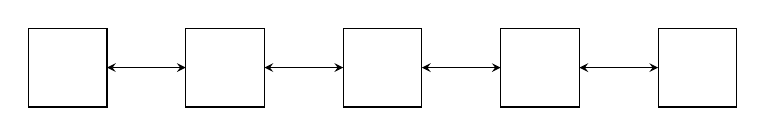
\begin{tikzpicture}
        %%%%%%%%%% Nodi %%%%%%%%%%
        \foreach \x in {0,2,...,8}
            \draw (\x,0) rectangle ++(1,1);

        %%%%%%%%% Frecce %%%%%%%%%
        \foreach \x in {1,3,...,7}
            \draw[<->,>=stealth] (\x,0.5) -- ++(1,0);
    \end{tikzpicture}
\end{center}

        \subsubsection{Lineare ad anello:}
            \begin{center}
    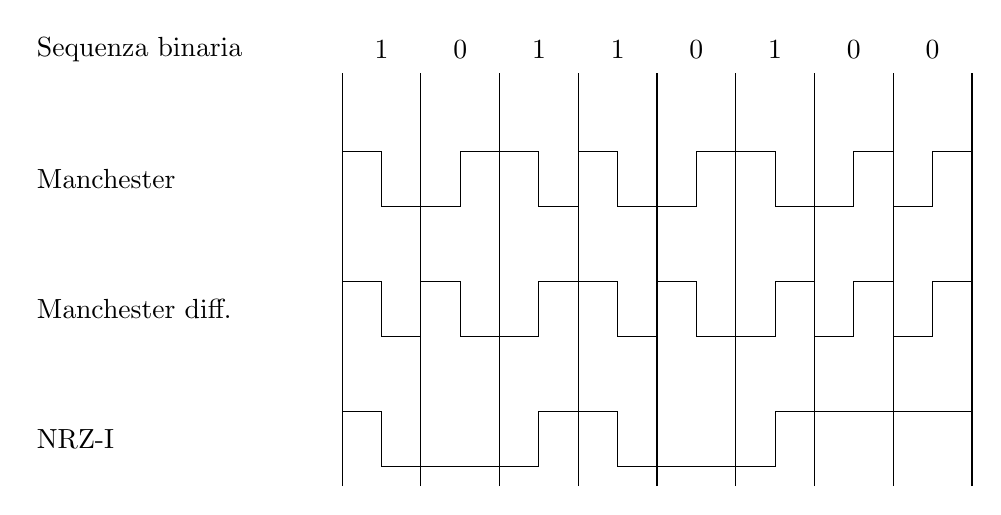
\begin{tikzpicture}
        %%%%%%%%% Barre %%%%%%%%%%
        \foreach \x in {4,...,12}
            \draw (\x,-0.25) -- (\x,5);

        %%%%%%%%% Numeri %%%%%%%%%
        \node at (4.5,5.3) {1};
        \node at (5.5,5.3) {0};
        \node at (6.5,5.3) {1};
        \node at (7.5,5.3) {1};
        \node at (8.5,5.3) {0};
        \node at (9.5,5.3) {1};
        \node at (10.5,5.3) {0};
        \node at (11.5,5.3) {0};

        %%%%%%%%% NRZ-I %%%%%%%%%%
        \draw (4,0.7) -- (4.5,0.7) -- (4.5,0) -- (6.5,0) -- (6.5,0.7) -- (7.5,0.7) -- (7.5,0) -- (9.5,0) -- (9.5,0.7) -- (12,0.7);

        %%%% Manchester Diff. %%%%
        \draw (4,2.35) -- (4.5,2.35) -- (4.5,1.65) -- (5,1.65);
        \draw (5,2.35) -- (5.5,2.35) -- (5.5,1.65) -- (6,1.65);
        \draw (6,1.65) -- (6.5,1.65) -- (6.5,2.35) -- (7,2.35);
        \draw (7,2.35) -- (7.5,2.35) -- (7.5,1.65) -- (8,1.65);
        \draw (8,2.35) -- (8.5,2.35) -- (8.5,1.65) -- (9,1.65);
        \draw (9,1.65) -- (9.5,1.65) -- (9.5,2.35) -- (10,2.35);
        \draw (10,1.65) -- (10.5,1.65) -- (10.5,2.35) -- (11,2.35);
        \draw (11,1.65) -- (11.5,1.65) -- (11.5,2.35) -- (12,2.35);

        %%%%%%% Manchester %%%%%%%
        \draw (4,4) -- (4.5,4) -- (4.5,3.3) -- (5,3.3);
        \draw (5,3.3) -- (5.5,3.3) -- (5.5,4) -- (6,4);
        \draw (6,4) -- (6.5,4) -- (6.5,3.3) -- (7,3.3);
        \draw (7,4) -- (7.5,4) -- (7.5,3.3) -- (8,3.3);
        \draw (8,3.3) -- (8.5,3.3) -- (8.5,4) -- (9,4);
        \draw (9,4) -- (9.5,4) -- (9.5,3.3) -- (10,3.3);
        \draw (10,3.3) -- (10.5,3.3) -- (10.5,4) -- (11,4);
        \draw (11,3.3) -- (11.5,3.3) -- (11.5,4) -- (12,4);

        %%%%%%%% Legenda %%%%%%%%%
        \node[anchor=west] at (0,5.3) {Sequenza binaria};
        \node[anchor=west] at (0,3.65) {Manchester};
        \node[anchor=west] at (0,2) {Manchester diff.};
        \node[anchor=west] at (0,0.35) {NRZ-I};
    \end{tikzpicture}
\end{center}

        \subsubsection{A stella}
            \begin{center}
    \begin{tikzpicture}
        %%%%%%%%%% Nodi %%%%%%%%%%
        \draw (0.8,0) rectangle (1.8,1);
        \draw (3.2,0) rectangle (4.2,1);
        \draw (0,2.2) rectangle (1,3.2);
        \draw (4,2.2) rectangle (5,3.2);
        \draw (2,4) rectangle (3,5);
        \draw (2,1.8) rectangle (3,2.8);

        %%%%%%%%% Frecce %%%%%%%%%
        \draw[<->,>=stealth] (1.3,1) -- (2,1.8);
        \draw[<->,>=stealth] (3.7,1) -- (3,1.8);
        \draw[<->,>=stealth] (1,2.8) -- (2,2.6);
        \draw[<->,>=stealth] (3,2.6) -- (4,2.8);
        \draw[<->,>=stealth] (2.5,4) -- (2.5,2.8);
    \end{tikzpicture}
\end{center}

        \subsubsection{Ad albero}
            \begin{center}
    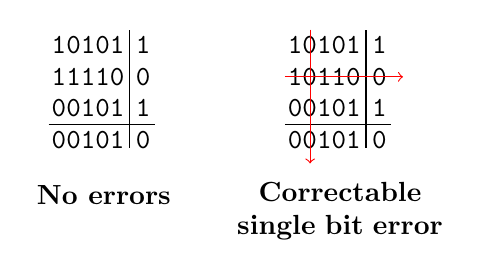
\begin{tikzpicture}
        %%%%%%%% Testo 1 %%%%%%%%%
        \node at (0,0) {\texttt{00101}};
        \node at (0,0.4) {\texttt{00101}};
        \node at (0,0.8) {\texttt{11110}};
        \node at (0,1.2) {\texttt{10101}};
        \node at (0.7,0) {\texttt{0}};
        \node at (0.7,0.4) {\texttt{1}};
        \node at (0.7,0.8) {\texttt{0}};
        \node at (0.7,1.2) {\texttt{1}};

        %%%%%%%% Schema 1 %%%%%%%%
        \draw (0.53,-0.1) -- (0.53,1.4);
        \draw (-0.5,0.2) -- (0.85,0.2);

        %%%%%%%% Testo 2 %%%%%%%%%
        \node at (3,0) {\texttt{00101}};
        \node at (3,0.4) {\texttt{00101}};
        \node at (3,0.8) {\texttt{10110}};
        \node at (3,1.2) {\texttt{10101}};
        \node at (3.7,0) {\texttt{0}};
        \node at (3.7,0.4) {\texttt{1}};
        \node at (3.7,0.8) {\texttt{0}};
        \node at (3.7,1.2) {\texttt{1}};

        %%%%%%%% Schema 2 %%%%%%%%
        \draw (3.53,-0.1) -- (3.53,1.4);
        \draw (2.5,0.2) -- (3.85,0.2);
        \draw[->,red] (2.5,0.8) -- (4,0.8);
        \draw[->,red] (2.82,1.4) -- (2.82,-0.3);

        %%%%%%%% Captions %%%%%%%%
        \node at (0.2,-0.7) {\textbf{No errors}};
        \node[text width=2.7cm,align=center] at (3.2,-0.9) {\textbf{Correctable single bit error}};
    \end{tikzpicture}
\end{center}

        \subsection{Completamente magliata}
            \input{chapters/1/assets/schema_e.tex}

        \subsection{Parzialmente magliata}
            \begin{center}
    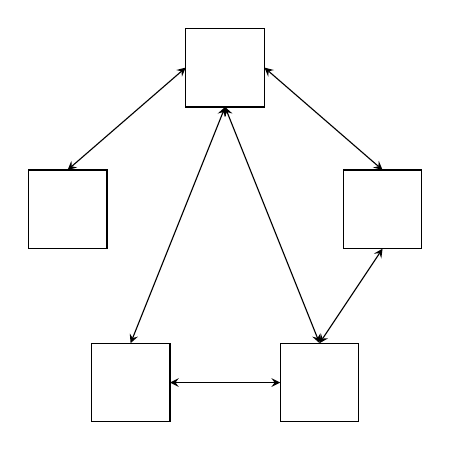
\begin{tikzpicture}
        %%%%%%%%%% Nodi %%%%%%%%%%
        \draw (0.8,0) rectangle (1.8,1);
        \draw (3.2,0) rectangle (4.2,1);
        \draw (0,2.2) rectangle (1,3.2);
        \draw (4,2.2) rectangle (5,3.2);
        \draw (2,4) rectangle (3,5);

        %%%%%%%%% Frecce %%%%%%%%%
        \draw[<->,>=stealth] (1.3,1) -- (2.5,4);
        \draw[<->,>=stealth] (1.8,0.5) -- (3.2,0.5);
        \draw[<->,>=stealth] (3.7,1) -- (2.5,4);
        \draw[<->,>=stealth] (3.7,1) -- (4.5,2.2);
        \draw[<->,>=stealth] (0.5,3.2) -- (2,4.5);
        \draw[<->,>=stealth] (4.5,3.2) -- (3,4.5);
    \end{tikzpicture}
\end{center}

        \subsubsection{A bus}
            \begin{center}
    \begin{tikzpicture}
        %%%%%%%%%% Nodi %%%%%%%%%%
        \foreach \x in {1,3,...,9}
            \draw (\x,0) rectangle ++(1,1);

        %%%%%%%%% Frecce %%%%%%%%%
        \draw[<->,>=stealth] (0,2) -- (11,2);

        \foreach \x in {1.5,3.5,...,9.5}
            \draw[<->,>=stealth] (\x,1) -- ++(0,1);
    \end{tikzpicture}
\end{center}

        \subsubsection{A griglia}
            \begin{center}
    \begin{tikzpicture}
        %%%%%%%%%% Nodi %%%%%%%%%%
        \node (HTTP) at (0,4) [draw,minimum width=2cm,minimum height=2em] {HTTP};
        \node (IMAP) at (3,4) [draw,minimum width=2cm,minimum height=2em] {IMAP};
        \node (FTP) at (6,4) [draw,minimum width=2cm,minimum height=2em] {FTP};
        \node (LDAP) at (9,4) [draw,minimum width=2cm,minimum height=2em] {LDAP};
        \node (TLS) at (4.5,2) [draw,minimum width=2cm,minimum height=2em] {SSL/TLS};
        \node (TCP) at (4.5,0.5) [draw,minimum width=2cm,minimum height=2em] {TCP};

        %%%%%%%%% Frecce %%%%%%%%%
        \draw[<->] (HTTP.south) |- ++(4.5,-0.6) -- (TLS);
        \draw[<-] (LDAP.south) |- ++(-4.5,-0.6);
        \draw[<-] (IMAP.south) -- ++(0,-0.6);
        \draw[<-] (FTP.south) -- ++(0,-0.6);
        \draw[<->] (TLS) -- (TCP);
    \end{tikzpicture}
\end{center}

    \newpage

    \subsubsection{Definizioni}
        \begin{itemize}
            \item \textit{Link}: canale di comunicazione che interconnette fisicamente due nodi. ogni link ha una propria ampiezza di banda e latenza.
            \item \textit{Path}: è la catena di link che compone un canale virtuale tra due nodi.
            \item \textit{Hops}: è il numero di link da attraversare.
            \item \textit{Path per link}: numero di path che possono attraversare un link.
            \item \textit{Diametro}: è il numero di hops tra i due nodi più lontani.
            \item \textit{Grado}: numero massimo di link connessi ad un nodo.
            \item \textit{Scalabilità}: capacità della topologia di sostenere più nodi.
        \end{itemize}

    \subsection{Commutazione di circuito e di pacchetto}
        Le reti vengono progettate secondo due possibili modelli di commutazione:
        \begin{itemize}
            \item \textbf{Commutazione di circuito} (tipicamente reti telefoniche)
            \begin{itemize}
                \item Viene individuato il percorso tra i due terminali e creato un circuito fisico temporaneo.
                \item Esiste un ritardo iniziale dovuto al tempio necessario per instaurare il circuito.
                \item I terminali scambiano i dati come se fosse un collegamento diretto.
                \item Il canale viene chiuso al termine della comunicazione.
            \end{itemize}

            \item \textbf{Commutazione di Pacchetto} (tipicamente reti dati)
            \begin{itemize}
                \item I dati della comunicazione sono frazionati in "pacchetti" con una lunghezza massima stabilita
                \item I nodi di transito (router, switch, etc.) hanno il compito di instradare ogni pacchetto.
                \item I pacchetti delle stessa comunicazione potrebbero seguire percorsi diversi.
                \item Il destinatario riassembla i pacchetti e ricostruisce il messaggio.
            \end{itemize}
        \end{itemize}

    \subsection{Modalità di trasmissione}
        Le comunicazioni sui canali possono essere:
        \begin{itemize}
            \item \textit{Simplex}: monodirezionali, esempio: TV.
            \item \textit{Half-duplex}: bidirezionali non simultanee, esempio: walkie-talkie.
            \item \textit{Full-duplex}: bidirezionali simultanee, esempio: telefono.
        \end{itemize}

    \subsection{Il modello ISO-OSI}
        A partire dal 1976 la \textbf{ISO (International Organization for Standardization)} ha dato il via a lavori per giungere ad un serie di standard unificati per la realizzazione di reti di calcolatori aperte.
        
        ISO ha proposto un modello di riferimento detto \textbf{OSI (Open System Interconnection)} che nel 1983 è diventato standard internazionale, esso viene comunemente detto ISO-OSI.

        Il modello ISO-OSI è basato sul concetto centrale di architettura a strati, la quale permette di scomporre il problema in sotto-problemi posti a diversi livelli, che sono più semplici da trattare ed independenti tra loro. I livelli del modello comunicano con quelli superiori e/o inferiori con interfacce standard, quindi strati diversi possono essere sviluppati da enti diversi.

        Il modello ISO-OSI scompone la comunicazione in sette livelli. Lo scopo di ogni livello, è quello di fornire servizi agli strati superiori, mascherando la loro implementazione. Ogni strato comunica logicamente con il pari stato del nodo remoto (\textbf{peer}), mentre comunica fisicamente con lo strato superiore ed inferiore dello stesso nodo.

        \subsubsection{Livello 1: Physic}
            Lo scopo del modello Fisico è la trasmissione dei bit grezzi sul canale di comunicazione, deve attivare, mantenere e disattivare la connessione fisica per conto del livello 2.
        
            Per fare queste operazioni, deve specificare le caratteristiche meccaniche (forma di prese e spine, numero dei contatti), elettriche (voltaggio e caratteristiche elettriche dei segnali associati all'interfaccia) e funzionali (significato dei vari segnali, schemi di codifica dei bit in grandezze fisiche).

        \subsubsection{Livello 2: Link}
            Il livello \textit{link} ha il compito di 
            \begin{itemize}
                \item Attivare, mantenere, disattivare la connessione fisica per conto del liv. 3.
                \item Rendere affidabile il collegamento diretto su un canale fisico.
            \end{itemize}

            Le funzioni tipiche di questo livello sono le seguenti:
            \begin{itemize}
                \item Strutturazione del flusso di dati in unità di dialogo, denominati \textbf{frames}.
                \item Controllo e gestione degli errori di trasmissione.
                \item Controllo di flusso (congestione).
                \item Controllo di sequenza (ordine).
            \end{itemize} 

            Per svolgere queste funzioni, viene aggiunta una intestazione (\textbf{header}) ad ogni frame, contenenete informazioni di servizio.
        
        \subsubsection{Livello 3: Network}
            Lo scopo dello strato di rete è di far giungere le unità d'informazione (\textbf{pacchetti}) al destinatario, determinando il path attraverso la rete.

            Si occupa del problema della commutazione, tramite la commutazione di pacchetto, cioè funzioni di \textbf{routing}.

        \subsubsection{Livello 4: Transport}
            Lo scopo del livello è fornire un canale sicuro end-to-end tra un processo mittente e destinatario, svincolando gli strati superiori da tutti i problemi di rete.

            Si occupa di frammentare i dati forniti dai livelli superiori; fornire una libreria API di programmazione, controllare il flusso, le congestioni, gli errori.

            Non tutte le applicazioni hanno bisogno delle stesse funzioni, per cui si possono definire delle classi di trasporto.

        \subsubsection{Livello 5: Session}
            Il livello \textit{session} suddivide il dialogo tra le applicazioni in unità logiche dette \textbf{sessions}.
        
            Una session deve essere individuata ed eventualmente interrotta e ripresa per far fronte a diversi problemi. Permette la chiusura ordinata del dialogo, con la garanzia che tutti i dati trasmessi siano arrivati a destinazione.

        \subsubsection{Livello 6: Presentation}
            Questo livello adatta il formato dei dati usato dai due interlocutori preservandone il significato.
        
            La descrizione del tipo di dati usati per un applicazione e del loro formato, si dice una sintassi.
        
            Ogni interlocutore ha bisogno di una sua sintassi locale per la rappresentazione dei dati e durante il dialogo bisogna concordare una sintassi di trasferimento. È stato definito un linguaggio ASN.1 (Abstract Syntax Notation 1) per descrivere e negoziare le sintassi.
        
        \subsubsection{Livello 7: Application}
            Lo strato di applicazione è l'utente della rete di calcolatori e pertanto non deve offrire servizi a nessuno.
        
            Rappresenta il programma applicativo, che per svolgere i suoi compiti ha bisogno di comunicare con altre applicazioni remote.

    \newpage
        
    \subsection{Svantaggi del modello ISO-OSI}
        Il modello ISO-OSI non ha avuto successo per vari motivi:
        \begin{itemize}
            \item Poca tempestività: le implementazioni di ISO-OSI sono arrivate quando ormai TCP/IP era già diffuso.
            \item Tecnologia scadente: ci sono livelli troppo vuoti (presentation e session) ed altri troppo pieni (data link e network).
            \item Implementazioni carenti: le prime implementazioni erano lente complicate ed enormi; al contrario, TCP/IP era semplice, veloce e soprattutto open.
            \item Incapacità politica: ISO-OSI è stato percepito come uno standard burocratico.
        \end{itemize}

    \subsection{Il modello TCP/IP}
        Il modello \textit{TCP-IP} è stato realizzato prima dell'ISO-OSI, ma standardizzato successivamente; ma poiché era già ampliamente diffuso, ISO-OSI rimane solo un modello di riferimento.

        \subsubsection{Livelli 1 e 2: Physic and Link}
            Per questi stati il modello TCP/IP non definisce nessun protocollo.
        
            Sono strati strettamente legati all'hardware di rete e vengono generalmente implementati nel device-driver della scheda e comunicano con i livelli superiori mediante una interfaccia standard.
    
            Abbiamo due famiglie di protocolli:
            \begin{itemize}
                \item I protocolli WAN ad esempio: HDLC e PPP.
                \item I protocolli LAN ad esempio: Ethernet.
            \end{itemize}

            I protocolli dello stato fisico assegnano ad ogni interfaccia un indirizzo specifico, denominato \textbf{indirizzo fisico}.

            Tutti questi protocolli ricevono il \textbf{payload} (carico utile) dal livello rete (pacchetto) che imbustano in un \textbf{frame} in cui viene aggiunta una intestazione (header) con campi necessari per il rilevamento degli errori, lo smistamento al livello superiore, l'indirizzamento.

        \subsubsection{Network}
            Lo strato rete ha il compito di mettere in comunicazione ed integrare tra loro diverse reti data-link. Richiede l'esistenza di particolari nodi, detti \textbf{router}, al confine tra 2 reti data-link, con il compito di "routare" da una rete all’altra solamente i pacchetti che ne hanno necessità.

            La suite di protocolli TCP/IP implementa questa funzionalità nel protocollo IP. Il protocollo IPv4 assegna ad ogni interfaccia di rete un indirizzo a 32 bit (4 byte) (indirizzo logico) che solitamente viene rappresentato mediante una sequenza di 4 numeri decimali separati da punto (.); ogni numero rappresenta un byte, per cui può assumere valori tra 0 e 255.

            I bit della sequenza sono suddivisi in due parti: la prima parte denominata \textit{network} è comune a tutti i nodi dello stessa rete LAN, mentre la seconda parte, denominata \textit{host}, distingue i nodi all'interno della LAN.

        \subsubsection{Livello 4: Transport}
            Questo strato fornisce una connettività diretta tra due nodi indipendentemente dal percorso fisico di collegamento, svincolando gli strati superiori da tutti i problemi di rete.
        
            Servizi offerti:
            \begin{itemize}
                \item \textit{Pacchettizzazione} (fragmenting/reassembling): il flusso di dati da spedire viene frazionato in segmenti che diventano il payload del pacchetti di livello rete.
                \item \textit{Multiplexing/demultiplexing}: Ad ogni applicazione verrà associato un numero di porta univoco sul nodo, in modo da distinguere i pacchetti provenienti dallo stato inferiore e dirottarli sull'applicazione corretta.
            \end{itemize}

            Diversi tipi di servizio in base alle necessità:
            \begin{itemize}
                \item Connection-Less, fornito dal protocollo UDP. Senza garanzia di ricevi- mento, senza riscontro, utilizzato da applicazioni che devono scambiarsi rapidamente brevi messaggi.
                \item Connection-Oriented, fornita dal protocollo TCP in cui viene attivato un canale virtuale tra le due parti. Il TCP fornisce la garanzia di consegna senza errori e il controllo del flusso.
                \item API: Le applicazioni del nodo potranno essere implementate per mezzo di una opportuna libreria di API, scegliendo il tipo di servizio più adatto alle proprie esigenze.
            \end{itemize}

            Visto che è possibile avere più applicazioni di rete sullo stesso nodo, il livello di trasporto fornisce un meccanismo di multiplexing e demultiplexing basato sul concetto di porta, \textbf{door}.

            Ad ogni applicazione verrà associato un numero di porta univoco sul nodo, in modo da distinguere i pacchetti provenienti dallo stato inferiore e dirottarli sull'applicazione corretta.

            La porta è un identificativo numerico (indirizzo di porta) che rappresenta il punto di arrivo di una connessione su di un host. La coppia (IPaddr, Port) identifica quindi univocamente un estremo di una connessione ed è detta \textbf{socket}.

        \subsubsection{Livello 5: Application}
            Il modello client-server richiede che sia ben identificabile e indirizzabile il server.

            Le porte TCP o UDP assegnate ad applicativi con ampia diffusione vengono as- segnate da un organismo internazionale (\textbf{IANA}) e prendono il nome di \textbf{Well Known Ports}.

            Contrariamente le porte dei client vengono determinate dinamicamente dal sistema operativo al momento dell'accesso al server.

            Ogni applicativo assegna ai propri oggetti un indirizzo specifico mnemonico.

    \subsection{Enti di standardizzazione}
        Esistono molti costruttori e fornitori di reti, ognuno con le proprie impostazioni. La necessità dell'interoperabilità richiede la presenza di standard condivisi per ogni aspetto della rete.

        Gli standard vengono proposti da diversi organismi internazionali, i principali sono:
        \begin{itemize}
            \item \textbf{ITU (International Telecommunication Union)} ha il compito di standardizzare le telecomunicazioni, principalmente telefoniche.
            \item \textbf{OSI (Open Standard Inteconnect)} definisce standard per una vasta gamma di argomenti. Sono stati emanati più di 17000 standard, incluso lo standard OSI.
            \item \textbf{IEEE (Institute of Electrical and Electronics Engineers)} è il principale ente professionale del mondo. Pubblica periodici, organizza conferenze ed emana standard nel campo dell'ingegneria elettrica e dei computers. Il comitato IEEE 802 ha standardizzato molti tipi di LAN.
            \item \textbf{ISoc (Intenet Society)} è nata nel 1992 su iniziativa di Vint Cerf and Bob Kahn per governare la crescita di internet. Gli standard sono emanati da IETF (Intenet Engineer Task Force) attraverso gli RFC (Request For Comment).
            \item \textbf{W3C (World Wide Web Consortium)} è un consorzio industriale guidato da Tim Bernes-Lee (creatore del web) che sviluppa protocolli e linee guida per la crescita a lungo termine del Web (HTTP, HTML, privacy, ecc).
        \end{itemize}